%! TEX root = 5_shearwall.tex
% the main TeX file which is intended to compile, :VimtexReload after adjustment
   % this file should be included in the main file
% :h vimtex-tex-root
\documentclass[../modul_skb.tex]{subfiles}
%ensure the class of docs

\begin{document}

\section{Dinding Geser (Shear Wall)}%
\label{sec:Dinding Geser (Shear Wall)}

Shear wall atau lebih dikenal dengan istilah dinding geser adalah element struktur berbentuk dinding beton bertulang yang berfungsi untuk menahan gaya geser, gaya lateral akibat gempa bumi atau gaya lainnya pada gedung bertingkat dan bangunan tinggi. Dinding geser ini terdapat berbagai jenis di dalam gedung antara lain bearing wall, frame wall, dan core wall. Pengertian shear wall dapat digambarkan sebagai berikut.


\begin{itemize}
	\item Bearing wall
	\item[] Bearing wall adalah jenis dinding geser yang mempunyai fungsi lain sebagai penahan beban gravitasi.
	\item Frame wall
	\item[] Frame wall adalah dinding geser yang berfungsi sebagai penahan gaya lateral, geser dan pengaku pada sisi luar bangunan. Dinding ini terletak di antara dua kolom struktur.
	\item Core wall
	\item[] Core wall adalah jenis dinding geser yang terletak di pusat-pusat massa bangunan yang berfungsi sebagai pengaku bangunan gedung. Biasanya core wall diletakkan pada lubang Lift yang berfungsi sebagai dinding lift sekaligus.
\end{itemize}

\begin{figure}
	\begin{center}
		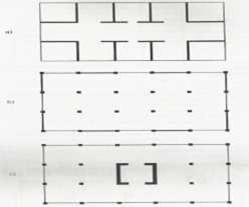
\includegraphics[width=.82\textwidth]{../figures/bear_wall.jpg}
		% filename may not contain space but _
	\end{center}
	\caption{(a) bearwing wall (b) framewall (c) core wall}
	\label{fig:mcm_shear}
\end{figure}


\begin{figure}
	\begin{center}
		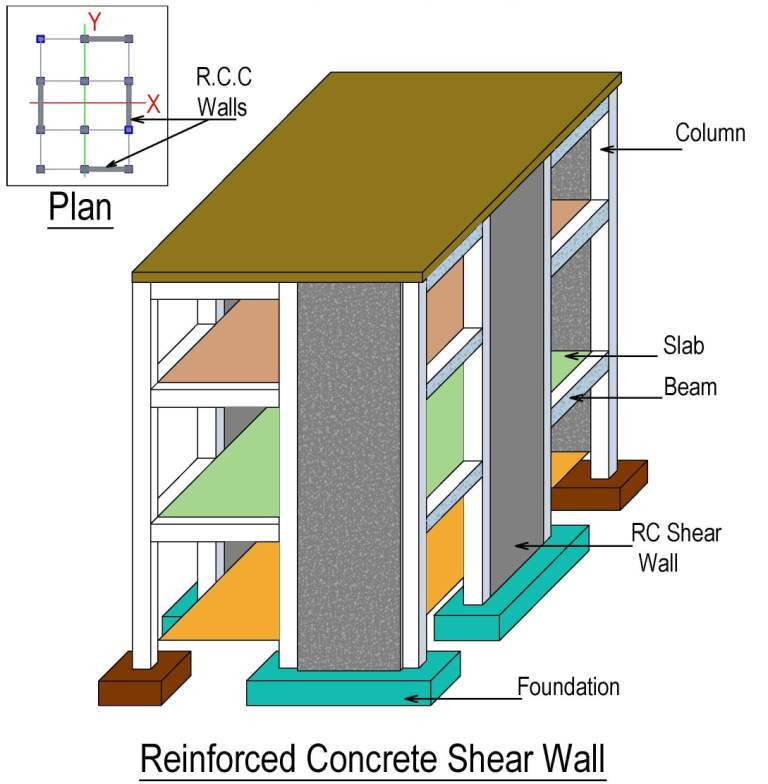
\includegraphics[width=.82\textwidth]{../figures/dinding_geser_beton_bertulang.jpg}
		% filename may not contain space but _
	\end{center}
	\caption{Dinding geser beton bertulang}
	\label{fig:shearwall}
\end{figure}

Letak shear wall pada bangunan gedung sangat tergantung dari beberapa faktor antara lain tingkat simetrisitas bangunan, tinggi bangunan, dan asumsi dari perencana. Penentuan lokasi dan perhitungan shear wall tentu dilakukan oleh perencana struktur dengan dasar-dasar perencanaan yang kuat. Shear wall pada gedung biasanya menggunakan mutu beton di atas \textit{Fc 30 Mpa}.


\subsection{Fungsi Shear Wall / Dinding Geser pada Bangunan}%
\label{sub:Fungsi Shear Wall / Dinding Geser pada Bangunan}

Berikut fungsi shear wall / dinding geser pada bangunan, yaitu:

\begin{itemize}
	\item Kekuatan
	\item[] Dinding geser harus memberikan kekuatan lateral yang diperlukan untuk melawan kekuatan gempa horizontal. Ketika dinding geser cukup kuat, mereka akan mentransfer gaya horizontal ini ke elemen berikutnya dalam jalur beban di bawah mereka, seperti dinding geser lainnya, lantai, pondasi dinding, lembaran atau footings.
	\item Kekakuan
	\item[] Dinding geser juga memberikan kekakuan lateral untuk mencegah atap atau lantai di atas dari sisi goyangan yang berlebihan. Ketika dinding geser cukup kaku, mereka akan mencegah membingkai lantai dan atap anggota dari bergerak dari mendukung mereka. Juga, bangunan yang cukup kaku biasanya akan menderita kerusakan kurang nonstruktural.
\end{itemize}

\subsection{Perilaku Struktur Rangka Kaku, Dinding Geser, dan Struktur Rangka- Dinding Geser (Dual System)}%
\label{sub:Perilaku Struktur Rangka Kaku, Dinding Geser, dan Struktur Rangka- Dinding Geser (Dual System)}

\subsubsection{Perilaku Struktur Rangka Kaku (Rigid Frame)}%
\label{ssub:Perilaku Struktur Rangka Kaku (Rigid Frame)}

Sistem rangka kaku atau rigid frame biasanya berbentuk rangka segi empat teratur yang terdiri dari balok horizontal dan kolom vertikal yang terhubung pada suatu bidang secara kaku (rigid), sehingga pertemuan antara kolom dan balok dapat menahan momen. Pada dasarnya rangka kaku akan ekonomis digunakan sampai 30 lantai untuk rangka baja dan sampai 20 lantai untuk rangka beton bertulang (Schueller, 1989). Karena sifat hubungan yang kontinuitas antara kolom dan balok, maka mekanisme rangka kaku dalam menahan beban lateral merupakan suatu respons bersama dari balok dan kolom, terutama respons melalui lentur dari kedua jenis elemen tersebut, seperti yang ditunjukkan pada gambar~\ref{fig:respon_lenturan}.

\begin{figure}
	\begin{center}
		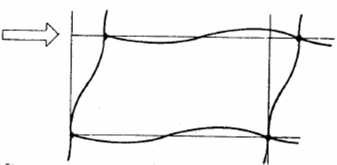
\includegraphics[width=.82\textwidth]{../figures/respon_lenturan.jpg}
		% filename may not contain space but _
	\end{center}
	\caption{Respon Lenturan Balok dan Kolom}
	\label{fig:respon_lenturan}
\end{figure}

Schueller (1989) menjelaskan bahwa lendutan lateral yang terjadi pada balok dan kolom pada struktur rangka kaku disebabkan oleh dua hal, yaitu:

\begin{itemize}
	\item Lendutan disebabkan oleh lentur kantilever
	\item[] Lenturan ini dikenal sebagai chord drift, yaitu dimana saat menahan momen guling (overturning moment) akibat beban lateral, struktur rangka beraksi sebagai suatu balok kantilever vertikal yang melentur dalam bentuk deformasi aksial dari kolom-kolom penyusunnya. Lentur kantilever ini kira-kira menyumbangkan 20\% dari total simpangan struktur.
	\item Deflaksi karena lentur balok dan kolom
	\item[] Perilaku struktur akibat lentur balok dan kolom dikenal sebagai shear lag atau frame wracking. Adanya gaya geser yang terjadi pada kolom dan balok akan menimbulkan momen lentur pada kedua elemen tersebut. Lenturan pada kolom dan balok menyebabkan terjadi distorsi secara keseluruhan pada rangka gedung. Tipe deformasi ini menyebabkan ± 80\% dari total simpangan struktur yang terdiri dari 65\% akibat lenturan balok dan 15\% akibat lenturan kolom.
\end{itemize}

\begin{figure}
	\begin{center}
		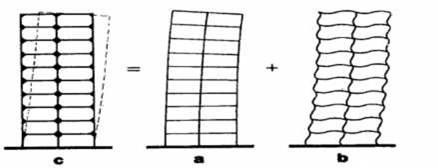
\includegraphics[width=.82\textwidth]{../figures/simpangan_rangka_kaku.jpg}
		% filename may not contain space but _
	\end{center}
	\caption{Simpangan pada Struktur rangka kau}
	\label{fig:simpangan_rigid}
\end{figure}

Pada gambar~\ref{fig:simpangan_rigid} menunjukkan suatu struktur rangka kaku yang menerima gaya lateral akan mengalami simpangan ke arah beban yang bekerja gambar~\ref{fig:simpangan_rigid}(c) , yang merupakan kombinasi simpangan yang diakibatkan oleh lentur kantilever ~\ref{fig:simpangan_rigid}(a) sebesar 20\% dari total keseluruhan simpangan dan lentur balok dan kolom ~\ref{fig:simpangan_rigid}(b) sebesar 80\% dari total keseluruhan simpangan (Schueller, 1989).

\subsubsection{Perilaku Dinding Geser (Shearwall/Cantilever Wall)}%
\label{ssub:Perilaku Dinding Geser (Shearwall/Cantilever Wall)}


Dinding geser merupakan suatu subsistem gedung yang memiliki fungsi utama untuk menahan gaya lateral akibat beban gempa. Keruntuhan pada dinding geser disebabkan oleh momen lentur karena terjadinya sendi plastis pada kaki dinding. Semakin tinggi suatu gedung, simpangan horizontal yang terjadi akibat gaya lateral akan semakin besar, untuk itu sering digunakan dinding geser pada struktur bangunan tinggi untuk memperkaku struktur sehingga simpangan yang terjadi dapat berkurang. Dinding geser juga berfungsi untuk mereduksi momen yang diterima struktur rangka sehingga dimensi struktur rangka dapat dibuat seefisien mungkin pada struktur bangunan tinggi akibat gaya lateral.
Gaya lateral yang terjadi pada suatu gedung, baik diakibatkan oleh beban gempa maupun angin akan disebar melalui struktur lantai yang berfungsi sebagai diafragma horizontal yang kemudian akan ditahan oleh dinding geser karena memiliki kekakuan yang besar untuk menahan gaya lateral (Shueller, 1989). Dinding geser dapat dianggap sebagai balok yang tebal karena kekakuannya dan berinteraksi terhadap gaya lateral serta lentur terhadap momen guling (overtuning momen). Kemampuan dinding geser dalam menahan gaya lateral, torsi, dan momen guling tergantung dari konfigurasi geometri, orientasi, dan lokasi dinding geser pada suatu bangunan.

\subsubsection{Perilaku Struktur Rangka-Dinding Geser (Dual System)}%
\label{ssub:Perilaku Struktur Rangka-Dinding Geser (Dual System)}

Semakin tinggi suatu gedung, penggunaan struktur rangka saja untuk menahan gaya lateral akibat beban gempa menjadi kurang ekonomis karena akan menyebabkan dimensi struktur balok dan kolom yang dibutuhkan akan semakin besar untuk menahan gaya lateral. Oleh karena itu, untuk meningkatkan kekakuan dan kekuatan struktur terhadap gaya lateral dapat digunakan kombinasi antara

rangka kaku dengan dinding geser (dual system). Pada struktur kombinasi ini, dinding geser dan kolom-kolom struktur akan dihubungkan secara kaku (rigid) oleh balok-balok pada setiap lantai bangunan. Dengan adanya hubungan yang rigid antara kolom, balok, dan dinding geser akan memungkinkan terjadinya interaksi antara struktur rangka dan dinding geser secara menyeluruh pada bangunan, dimana struktur rangka dan dinding geser akan bekerja bersama-sama dalam menahan beban yang bekerja baik itu beban gravitasi maupun beban lateral. Selain itu, dengan menggunakan sistem ganda ini, maka simpangan lateral akan jauh berkurang seiring dengan peningkatan jumlah lantai struktur. Semakin tinggi suatu struktur gedung, semakin kecil simpangan yang terjadi. Besarnya simpangan keseluruhan yang terjadi pada sistem rangka kaku-dinding geser diperoleh dengan cara menggabungkan perilaku kedua elemen tersebut seperti yang terdapat pada gambar~\ref{fig:superimposmode}.

\begin{figure}
	\begin{center}
		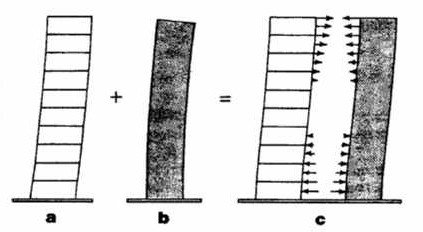
\includegraphics[width=.82\textwidth]{../figures/deformasi_shear.jpg}
		% filename may not contain space but _
	\end{center}
	\caption{Superimpos mode individu dari deformasi}
	\label{fig:superimposmode}
\end{figure}


\begin{itemize}
	\item Deformasi mode geser untuk rangka kaku (gambar~\ref{fig:superimposmode}(a))
	\item[] Pada struktur rangka kaku, sudut deformasi (lendutan) paling besar terjadi pada dasar struktur dimana terjadi geser maksimum.
	\item Deformasi mode lentur untuk dinding geser (gambar~\ref{fig:superimposmode}(b))
	\item[] Pada struktur dinding geser, sudut deformasi (lendutan) paling besar terjadi pada bagian atas bangunan sehingga sistem dinding geser memberikan kekakuan paling kecil pada bagian atas bangunan.
	\item Interaksi antara rangka kaku dan dinding geser (gambar~\ref{fig:superimposmode}(c))
	\item[] Interaksi antara struktur rangka kaku dan dinding geser diperoleh dengan membuat superposisi mode s defleksi terpisah yang menghasilkan kurva S datar. Perbedaan sifat defleksi antara dinding geser dan rangka kaku menyebabkan dinding geser menahan simpangan rangka kaku pada bagian bawah, sedangkan rangka kaku akan menahan simpangan dinding geser pada bagian atas. Dengan demikian, geser akibat gaya lateral akan dipikul oleh rangka pada bagian atas bangunan dan dipikul oleh dinding geser dibagian bawah bangunan.
\end{itemize}

\subsection{Metode Pelaksanaan Shear Wall}%
\label{sub:Metode Pelaksanaan Shear Wall}

\begin{itemize}
	\item Fabrikasi pembesian dinding shear wall.
	\item Pemasangan tulangan vertikal yang dicor bareng dengan pelat lantai bawahnya.
	\item Pemasangan tulangan horizontal, ikat dengan bendrat.
	\item Untuk area basement silahkan diberi waterstop untuk mencegah masukknya air.
	\item Pemasangan bekisting pada dua sisi luar. Pada bekisting diusahakan menggunakan as drat untuk mengunci dua bekisting agar tidak terjadi beton yang bunting.
	\item Cor beton dengan ready mix
	\item Bongkar bekisting
\end{itemize}

Element shear wall mempunyai pengertian yang hampir sama dengan element struktur lainnya yaitu untuk menahan gaya yang bekerja pada bangunan gedung. Sejauh ini penggunaan shear wall lebih banyak digunakan pada bangunan high rise building karena semakin tinggi bangunan semakin besar gaya gempa yang bekerja pada bangunan.







\bibliographystyle{apalike}
\bibliography{../filename.bib} % required for citecompletion, not work in mainfile
\end{document}

